\documentclass[12pt, a4paper]{article}
\usepackage{caption}
\usepackage{graphicx}
\usepackage{hyperref}
\hypersetup{
    colorlinks,
    citecolor=black,
    filecolor=black,
    linkcolor=black,
    urlcolor=black
}
\usepackage{tikz-network}
\usepackage{amsmath, amsfonts, amssymb, amsthm}
\usepackage{algpseudocode}
\usepackage{algorithm}
\title{Network and Cybersecurity}
\date{2022}
\author{Kristoffer Klokker}

\usepackage{xcolor,listings}
\usepackage{textcomp}
\usepackage{color}
\usepackage{listings}
\definecolor{codegreen}{rgb}{0,0.6,0}
\definecolor{codegray}{rgb}{0.5,0.5,0.5}
\definecolor{codepurple}{HTML}{C42043}
\definecolor{backcolour}{HTML}{F2F2F2}
\definecolor{bookColor}{cmyk}{0,0,0,0.90}  
\color{bookColor}

\lstset{upquote=true}

\lstdefinestyle{mystyle}{
    backgroundcolor=\color{backcolour},   
    commentstyle=\color{codegreen},
    keywordstyle=\color{codepurple},
    numberstyle=\numberstyle,
    stringstyle=\color{codepurple},
    basicstyle=\footnotesize\ttfamily,
    breakatwhitespace=false,
    breaklines=true,
    captionpos=b,
    keepspaces=true,
    numbers=left,
    numbersep=10pt,
    showspaces=false,
    showstringspaces=false,
    showtabs=false,
    tabsize=3,
}
\lstset{style=mystyle}
\usepackage{zref-base}

\makeatletter
\newcounter{mylstlisting}
\newcounter{mylstlines}
\lst@AddToHook{PreSet}{%
  \stepcounter{mylstlisting}%
  \ifnum\mylstlines=1\relax
    \lstset{numbers=none}
  \else
    \lstset{numbers=left}
  \fi
  \setcounter{mylstlines}{0}%
}
\lst@AddToHook{EveryPar}{%
  \stepcounter{mylstlines}%
}
\lst@AddToHook{ExitVars}{%
  \begingroup
    \zref@wrapper@immediate{%
      \zref@setcurrent{default}{\the\value{mylstlines}}%
      \zref@labelbyprops{mylstlines\the\value{mylstlisting}}{default}%
    }%
  \endgroup
}

% \mylstlines print number of lines inside listing caption
\newcommand*{\mylstlines}{%
  \zref@extractdefault{mylstlines\the\value{mylstlisting}}{default}{0}%
}
\makeatother


\newcommand\numberstyle[1]{%
    \footnotesize
    \color{codegray}%
    \ttfamily
    \ifnum#1<10 0\fi#1 |%
}


\begin{document}
	\maketitle
	\clearpage
	\tableofcontents
	\clearpage
	\section{Computer networks}
		A system connected to the internet is called a \textbf{host / end system}. This is done thorugh a \textbf{communication link} and \textbf{packet switch}. By this it has a \textbf{transmission rate} which describe the speed measured in bits/second.\\
		When data is send it is done through \textbf{packets} which consist of a data header and including data. A packet is send first to the packet switch often taking form of a router or link-layer-switch. Which then sends it further to the communication link.\\
		ISP then interconnect the communication links and connects to a higher up ISP or between higher up IPS. The highest tier is tier 1 of which other ISP connect with, even multiple such a \textbf{multi-home} setup is done in case of failure. An ISP may alos connect to a \textbf{PoP} which simply are a group of routers from another ISP.\\
		ISPS may also peer between eachother to reduce exhange with higher tier ISP and reduce cost. Most often are peering free and third party companies may even create a IXP where multiple ISP can connect and peer to each other.\\
		Big companies like Google also has their own private network infrastructure, which spans the globe between their datacenters. They are therefore peering between same tier ISPs and are also connected to 1 tier ISP but with reduced exhange.\\
		Edge network refers to the connections to all the end host.
		\subsection{Different types of connections}
			Home access can be done in different ways:
			\begin{itemize}
				\item DSL - Digital subscriber line is done through a telephone lines in higher frequencies such phone and network can coincide. Current max limit of downstream is 1 Gbps, but the whole system require small distance to the telco provider 8 - 16 km.
				\item Cable internet access - Internet done through the existing television coax cable or hybrid fiber coax (HFC), a modem is then used to translate the analog signal to digital signal. This allows up to 1.2 Gbps downstream. 
				\item FTTH - Fiber to the home is a direct connection from the cable office to the home. Here are two types active optical network (AON) and passive optical network (PON), PON works such a netowk teminator at the home goes through a splitter between up to 100 homes into the terminator at the telco.\\
				\item 5G fixed wireless - This is a wireless solution which are beginning to gather popularity in cities.
			\end{itemize}
			At the home a Local Access Network is then created, and most often extended to a Wireless Local Access Network using a router usin the WiFi protocol.
		\subsection{Mediums of signals}
			When a signal is sent through a physical media it is called guided media whereas over a wireless media it is called unguided.\\
			Example of mediums are:
			\begin{itemize}
				\item Twisted cobber wire - used for telephone connections an still in use, for ethernet and more. A communication link done with this is called unshielded twisted pair (UTP). Modern cables of category 6a can transfer up to 10 Gbps over hundreds of meters.
				\item Coaxial cable - much like the twisted cobber cable, but the two copper condctors work concentric rather than parallel.
				\item Fiber Optics - Works by sending light insted of electricity, can have speeds in up to hundreds of Gbps over distances up to 100km due to no electromagnetic interference.
				\item Terrestrial Radio Channels - radio signals which characteristics depend a lot on enviremental factors. Can be found in three categories, short distance up to 2 meters, medium distance up to a few hundred meters and long distance spanning tens of kilometers.
				\item Satellite Radio Channels - Works as a transmitter receiver between two points on earth. Either in a geostationary orbit or low-earth orbit. geostationary eliminate the need of always finding the optimal satelite but at consequence of 280 ms delay.
			\end{itemize}
		\subsection{Packet switching}
			Most packet switches use \textbf{store-and-forward transmission}, such before forwarding a transmittion all packages has to be obtained and proccessed before transmissioning.\\
			This therefore extend the tranmission time according to package number and speed. \\
			When the router has processed all packages they can be send as one unit.\\
			This therefore can be described with:
			$$d_{end-to-end}=N\frac{L}{R}$$
			Where $N$ is number of links, $L$ is number of bits in a package and $R$ is the speed.\\[4mm]
			In case of a package is alreadyu being sent the new package is sent to the \textbf{output buffer}, and in case of a full buffer \textbf{packet loss} will occur.\\
			A packet switch most often have multiple queues for different forwarding packages. The packages are placed based on a forwarding map, using the packages IP addres.
		\subsection{Circuit switching}
			A circuit switch networks works on reservations. Instead if queues, a reservation is made to the receiver in both bandwith and that a port is open for the package.\\
			This also has the advantage that the number of links can be ignored, in transmission time.\\
			In this way a package can be guranteed to come at a specific time and no lost of any package.\\
			To route more connections either \textbf{frequency-division multiplexing} or \textbf{time-division multiplexing} can be used.\\
			FDM splits the avaliable frequecies into smaller bandwith of which data can be sent through.\\
			TDM splits up the full bandwith into frames which are reserved with a number a number of slots for data. Therefore the speed is dependent on frame rate multipled by number of bits in a slot.\\
			The downside of circuit switching compared to package switching, is the need for allocated sapce for every user, even in inactivity whereas package switching can work with changing demand.
		\subsection{Delay}
			There are different kind og delays the most important are:
			\begin{itemize}
				\item Nodal processing delay - delays in the router such as determine package header or bit error correction ($\mu$s)
				\item Queuing delay - delays in case of heavy traffic and non empty buffers ($\mu$s - ms)
				\item Transmission delay - delays that occur when waiting for a whole package and transmission rate is low  ($\mu$s - ms) - $d_{trans}=\frac{L}{R}$
				\item Propagation delay - delays from the actual bit transportation limit by medium (ms) - $d_{prop}=\frac{m}{s}$
			\end{itemize}
			These in total are the total nodal dealy.\\
			
		\subsection{Protocols}
			A protocol defines the format and the order of messages exchanged between two or more communicating entities, as well as the actions taken on the transmission and/or receipt of a message or other event.\\[4mm]
			Protocols are therefore used everywhere, such everything works as expected in between the layers of the network.\\
			When different layers of protocols work together it is called a protocol stack, this may be for the internet: 
			\begin{itemize}
				\item Application - These are protocols which are sent pr apllication such as HTTP, SMTP, DNS and such, refered as message
				\item Transport - These protocols are for sending application messages, here TCP and UDP, refered as segment
				\item Network - Protocols for distributing the segments using IP protocols or other routing protocols therefore refered as IP layer
				\item Link - Protocols here are used for the IP layer to transmit to until reaching the physical layer, this is protocols such as Ethernet and WiFi, refered as frames
				\item Physical - Protocols for transmitting frames, here protocols depend on medium such as for fiber
			\end{itemize}
			When data goes through each layer, a new header is added and previus layer data is used as payload.\\
		\subsection{Network attacks}
			Some of the different kind of internet attacks include:\\
			Denial of service attacks (DoS) which prevent access to network host or infrastructure.\\
			It can work by 3 ways:
			\begin{itemize}
				\item Vulnerability attack - Few messages which use a exploit such the host either stops or crashes
				\item Bandwith flooding - A large amount of packages is sent to the host resulting in overfilled buffers
				\item Connection flooding - A large number of open TCP connections are made such every entry is occupied
			\end{itemize}
			For flooding attacks they may also be a distributed Dos  (DDoS) attack thorugh multiple devices often in a botnet.\\[4mm]
			A packet sniffer is a type of passive attack of which a device will listen for packages and possibly find sensitive information in packages sent through it.\\
			IP Spoofing is a package which source address is spoofed, and therefore faked to look as a different source.\\
	\section{Protocol layers}
		For an application communicates to network layer, a socket is setup, which indentifies by a port.
		An app-layer protocol defines
		\begin{itemize}
			\item Messages exchanges - requst, resonse,...
			\item Message syntax - what fields are in a message
			\item Message sematics - Meaning of fields
			\item Rules for send and reponds
		\end{itemize}
		Transport service requirements - The different requirements an application may set for the transport of data\\
		The different types of requirements an application may set
		\begin{itemize}
			\item Data loss - May be strictly no loss or just some percentage
			\item Throughput - May need a constant throughput or can be elastic 
			\item Time sensitive - May need a minimum latency for data
			\item Security - Some data may be more sensitive than other
		\end{itemize}
		\subsection{Client server architecture}
			The server side is on a always on host, with permanent ip, which handles backend stuff. \\
			Ex. are hosting api and database.\\
			The client in this architecture communicates via HTTP protocols are some alike.\\
			The clients are the dynamic part, may not be on same ip, or connect with each other\\
		\subsection{P2P}
			No host involved but clients communicating directly between each other.\\
			Are scaled based on number of users.
		\subsection{TCP Service}
			Reliable transport with flow control to not overwhelm receiver\\
			Able to throttle sender in an overloaded network.\\
			Does not provide: timing, min. througput guarantee or security\\
			Need a setup between client and server established before use.
		\subsection{UDP}
			Unreliable data transfer.\\
			Does not provide: reliability, flow control, congestion control, timing, throughput guarantee, security\\
			Smarter for data which can handler larger loss. \\
			TCP may get stuck on a packet whereas UDP would simply skip the package and go forward for the next package.\\
			UDP is also faster and connectionless therefore making it possible to handle more connections faster.\\
			The header includes 4 16 bits data: sorce port, destination port, length of data, checksum\\
			The checksum works by the data is split up into 16 bit words, then they are summed and overflow is wrapped around. Then the sum is converted to 1s compliment (everything is flipped). This will then be the checksum.\\
			If the checksum fails the data is either discarded or delivered with an error.
		\subsection{Domain name system}
			DNS binds name/string to an ip address.\\
			This also includes alias names for mail server or sub domains.\\
			Usefull for more dynamic ip setup and readability\\
			Implemented via a distributed database.\\
			The databases stores resource records (RR) in the format (name,value,type,ttl)\\
			The DNS is implemented in a tree structure.\\
			First are the root DNS which contains addresses of top level domain severs like .com, .org, .dk\\
			They then contain then the DNS servers for domain such as google.com, which itself contains addresses for subdomain.\\
			So when a request is made first, the cache is checked, then a request to a preinstalled root such as 1.1.1.1 is made.\\
			This then returns a top level address for a DNS server, which a request is made to. \\
			This is repeated until an ip matching the request is returned.\\
			This is the itterative method.\\
			The recursive query find the ip via the DNS servers which contacts eachother putting the burden on them\\
			Local DNS servers does not belong to hierarchy but is hosted by an ISP.\\
			TTL (time-to-live) is a numerical value representing the amount of server hops a packet can make before being outdated.\\	
			The local DNS handles the requesting and caching for an IP to the hiarachy DNS servers.
			\subsubsection{Types of resource records}
				To do a lookup the dig tool can be used
				\begin{itemize}
					\item Type=A - name: hostname, value: ip-address
					\item Type=NS - name: domain, value: nameserver
					\item Type=CNAME - name: alias, value: hostname
					\item Type=MX: name: '@', value: mail server
				\end{itemize}
			\subsubsection{DNS protocol}
				Query and reply are in the form Message, header\\
				The header consist 12 bytes dedicated to
				\begin{itemize}
					\item 16 bit identificaiton
					\item 16 bit flags
					\begin{itemize}
						\item Query (0) or reply (1)
						\item 4 bit opcode: standard query (0), domain name form ip (1), status request of server (2), (3) is reserved for status an not used
						\item AA: The server is authoritative (1), non authoritative/cache (2)
						\item TC: the message exceeds 512 bytes and are truncated (1)
						\item RD: Recursion desired (1)
						\item RA: Recursion avaliable from server (1)
						\item Zero: 3 bits of zeros reserved
						\item rCode: Respnse code, no error (0), format error (1), server failure (2), did not find name (3), request is supported (4), policy denies execution of query (5)
					\end{itemize}
					\item 16 bit Number of questions in body
					\item 16 bit Number of answers RRs and is 0 from client and set by server 
					\item 16 bit Number of authority RRs and is likewise 0 from client
					\item 16 bit Number of additional RRs 
				\end{itemize}
				The body then cosist of
				\begin{itemize}
					\item Questions - query from client
					\item Answers RRs- Response to query from non authority
					\item Authority RRs -  Response to query from authority
					\item Additional information 
				\end{itemize}
			\subsubsection{Security}
				A person could bombard the DNS servers with traffic and deny other trafffic in form of DDoS.\\
				Not successful to date on root server but TLD (top-level domain) has successed\\
				NXDOMAIN attack is requesting non existing domains and spending the DNS server ressources to find non valid addresses.\\
				Random subdomain attack are like NXDOMAIN attack but with subdomains to target the namespace rather than root or TLD.\\
				Phantom domain attack is setting up DNS servers which does not respond or very slow responses, such in a recursive lookup the TLD will have to wait for response.\\
				TCP SYN is the attack of which a bunch of TCP request are opened but never used.\\
				DNS domains lock-up is an extended TCP SYN attack where after a connection is established random packages is sent to the server, and the server will wait for a correct response.\\
				DNS rebinding attack is used to get past browsers same-origin policy, this is done by first the user lands on a shady website, the website then make a request to itself, but the dns record is updated to point at a new site which the script now can be run upon.\\
				DNS cache poisoning is where an attacker imposes as a nameserver, and then creates a request for the nameserver and answers before the real nameserver and thereby creating a fake lookup in the cache.
	\section{Web and HTTP}
		\subsection{HTTP}
			A HTTP request is sent by the client, and server sends using HTTP protocol an object in response\\
			The request is sent at port 80 using a TCP request.\\
			Non-persistent HTTP sendt a single object and then closes\\
			Persisten HTTP can send multiple files between client and server\\
			Repsonse time RTT is the time for a small packet to travel from client to server and back.\\
			Persistent has longer open connection but every referenced object can be sent at as little as one RTT\\
			Non-persisten requires 2 RTT atleast pr referenced object, and looses alot of time to OS overhead for each established connection.\\[4mm]
			The general request consist of: method, url, protocol, headers\\
			The general response consit of: protocol, status code, status phrase, headers, data\\
			There is 4 method types for HTTP/1.1
			\begin{itemize}
				\item GET - get ressource
				\item POST - send ressource
				\item HEAD - meta data to check for updates
				\item PUT - Uploads file in entity body to url field
				\item DELETE - delete file in the url field
			\end{itemize}
			The most common response status codes
			\begin{itemize}
				\item 200 OK
				\item 301 Moved Permanently - object is moved to new location given in message
				\item 400 Bad Request - not understood by server
				\item 404 Not Found - Fil not found on server
				\item 505 HTTP version not supported 
				\item 418 I'm a teapot - When a teapot is requested to bre coffee
			\end{itemize}
		\subsection{Cookies}
			Cookies are the solution for http being stateless.\\
			Cookies allows to store files in the browser of the user.\\
			This can be used for saved storage like shopping cart or authority like a session cookie.\\
		\subsection{HTTP/2.0}
			Problem in 1.0 was request was treated in order, 1.1 made it a little better using pielining which allowed for multiple sequential request.\\
			2.0 introduced streams, where request are numbered in odds and responses are given in even numbers.\\
		\subsection{Electronic mail}
			Electronic mail consist of 3 major components: User agents, Mail servers and Simple mail transfer protocol (SMTP)\\
			User agents are essentially mail clients which allows for creation and reading of emails.\\
			Mail servers have a mailbox for incomming messages and a message queue for outgoing mails\\
			SMTP uses TCP on port 25 to transfer emails.\\
			The protocol work on command response, where command are in ASCII 7 bit and reponse are status codes.\\
			The mail message consist of header (To, from, subject), blank line and body (Only ASCII)\\
			The user agents access the mail server via the IMAP protocol or HTTP\\
		\subsection{Video streaming and content delivery networks}
			To reduce the amount of data, coding is used on the data, spatial (groups pixels together) and temporal (only send difference of video frames)\\
			CBR - constant bit rate\\
			VBR - variable bit rate\\
			DASH - Dynamic, Adaptive Streaming over HTTP\\
			DASH divides video files into chunks, with each having different rates.\\
			All chunks are managed in the manifest file which provides URL to each chunk.\\
			The client then handles, when to get chunks, at what encoding rate and which server to request chunks.\\
			CDN networks work by distributing the content to multiple servers around the globe.\\
			To find the best server in a CDN preiod tests are made in the network of which speeds are in between each server.\\
		\subsection{P2P}
			No need for an always on server\\
			End systems directly communicate.\\
			Is more scaleable than a server setup.\\
			For $n$ clients on a server the sever time will be $D_{Client-Server}>max(NF/u_s,F/d_{min})$, it will therefore scale linearly.\\
			Whereas in P2P the time will be $D_{P2P}>max(F/u_s,F/d_{min},NF/(U_s+\sum u_i))$\\
			Where $U_s$ is the central server speed, $u_i$ is user upload speed, $d_i$ user download speed and $F$ is filesize.\\
			A torrent is a group of peers exchaning files divided into chunks of 256Kb.\\
			The peers are then managed in a tracker, which also participate in the torrent.\\
			A torrent client then uses those peers, request which chunks they have and missing chunks are downloaded from fastest connection.\\
	\section{Network security}
		The properties of secure communication
		\begin{itemize}
			\item Confidentiaity - Only sender and reciever should be able to read the message using encryption
			\item Message integrity - The message should not be altered by intent or accident which is checked using check sum
			\item End-point authentication - Insuring sender and reciever are able to confirm their idenitity
			\item Operational security - A firewall or depp packet inspection may be setup between local network and public network to counter malicious attacks
		\end{itemize}
		\subsection{Principles of crypthography}
			A text is first plain text and after using the encryption algorithm it becomes a ciphertext.\\
			The most used method used today are based on keys between sender an receiver.\\
			The a symmetric key system both sender and receiver has to same key to decrypt an encrypt.\\
			In a public key system sender and receiver has 2 keys a public $K^+$ and private $K^-$. The sender then encrypts using the public receiver key which then can be decrypted by the receiver using the private key.\\
		\subsection{RSA}
			RSA is an algorithm to implement public key system.\\
			To generate a public and private key the following is done
			\begin{itemize}
				\item Two large primes are choosen to larger to higher encryption though longer de,- and encryption times, but the product should be in the order of 1024 bits
				\item Computer $n=pq$ and $z=(-1)(q-1)$
				\item A number $e$ is choosen which is $e<n$ and $gcd(e,n)=1$
				\item Find a number $d$ such $ed-1 \mod z=1$ 
				\item $K^+=(n,e)$ and $K^-=(n,d)$
			\end{itemize}
			The encryption $c$ is then done by
			$$c=m^e\mod n$$ where $m<n$\\
			The decryption is then done by
			$$m=c^d\mod n$$
			This does take a lot of data and time therefore often sessions keys are generated and shared using RSA.\\
			This works by when a message is encrypted and decrypted it is expressed as
			\begin{align}
				m&=(m^e\mod n)^d\mod n\\
				&=m^{ed}\mod n\\
				&=m^{ed\mod z}\mod n\\
				&=m^1\mod n\\
				&=m
			\end{align}
			(2) can be done as proberty of modulo. (3) is possible because be definition $p$ and $q$ are prime and $n=pq$ and $z=(p-1)(q-1)$ makes it such $x^y$ mod $n=x^{y\;\text{mod}\;x}$.\\
			(4) can be done due to $z$ was choosen by definition to be $ed\mod z = 1$. (5) is done since $m<n$.\\
			Since $e$ and $d$ are multiplied we would get the same result if the message is encrypted or decrypted first.\\[4mm]
			The safety of RSA relies on there is no known fast factoring of number alogirthm
			
		\subsection{Symmetric key encryptions}
			\begin{itemize}
				\item Caesar cipher - Every letter is shifted a number in the alphabet with wrap araound
				\item Monalphbetic cipher - Every letter is mapped to another letter
				\item Polyalphabetic - Using multiple monoalphabetic ciphers in a certain order
				\item Block cipher (ECB) -  The message is split up into blocks of size $k$ which then is mapped to an encrypted block in same size
				\item Advanced block cipher (OFB) - Split message up to smaller block of size $k_1$ and then again to size $k_2$, the $k_2$ is then scrambled in place. This is repeated $n$ times
				\item Cipher block chaining (CFB) - First a Initization vector is genereated and send, then every block is XOR'ed with the last send message and encrypted using shared key.
			\end{itemize}
			To attack a simple encryption there are different methods
			\begin{itemize}
				\item Ciphertext-only attack - Can be attacked using statistical analysis
				\item Known-plaintext attack - If some of the plaintext is known and therefore can be matched to the encryption
				\item Chosen-plaintext attack - If the attacker has access to the plaintext and can therefore get information about the encryption
			\end{itemize}
			\subsubsection{Feistel cipher}
				\begin{figure}[h!]
					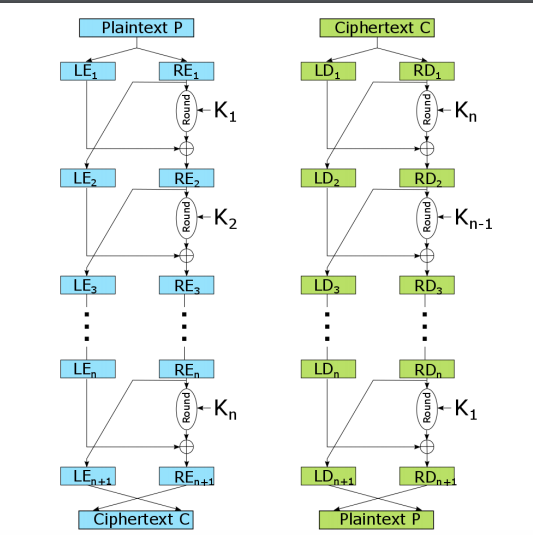
\includegraphics[width=300px]{assets/feistelCipher.png}
					\centering
					\caption{Feistel cipher illustration by \href{https://crypto.stackexchange.com/questions/67717/learning-about-feistel-cipher}{terodee}}
				\end{figure}
				The cipher works by
				\begin{enumerate}
					\item Plaintext is splitted into 2 chunks left and right
					\item A function is then performed on the right using key 1
					\item The left chunk is then XOR'ed with the output of the function
					\item The XOR output is now the right chunk and the original right chunk is the left chunk
					\item 2 - 3 is repeated $n$ times with the last chunk as input and the key is itterated
					\item Left and right are switched
				\end{enumerate}
				To then decrypt the same algorithm is used with the reverse order of the keys.\\
				This will work due to XOR being reversible
			\subsubsection{DES}
				A symmetric encryption system, such input and output are the same size\\
				First the plaintext is divided into 64 bit chunks.\\
				A 64 bit key is generated.\\
				Then an inital permutation is done on the 64 bit text using a predetermined vector of value mappings.\\
				A feistel cipher is then done with 16 rounds, where the function is defined as:\\
				\begin{enumerate}
					\item The 32 bit input is expanded to 48 bit 
					\item The 48 bit is XOR'ed using the input key 
					\item The 48 bit is then substituted using the S-Box table to 32 bits. This is done by splitting the 48 bits into 6 bits chunks. Then bit 1 and 6 is the row number and 2,3,4 and 5 is the column number.
					\item The 32 bits are then permutated using the P-table.
				\end{enumerate}
				After the feistel cipher, a final permutation is done by with the inverse of the first permutation.\\[4mm]
				To find the subkeys for each of the 16 rounds the following is done to the key.\\
				First the key is reduced to 56 using permuted choice 1 table, where two chunks of 28 is created is also divided.\\
				Each chunk is then circular left shifted once on itteration 1,2,9 and 16 and shifted twice on every other itteration.\\
				Then the second permutation table is used to generate the 48 bit sub key.\\
				By this method a bit will be used in 14 out of the 16 keys.
				\begin{figure}[h!]
					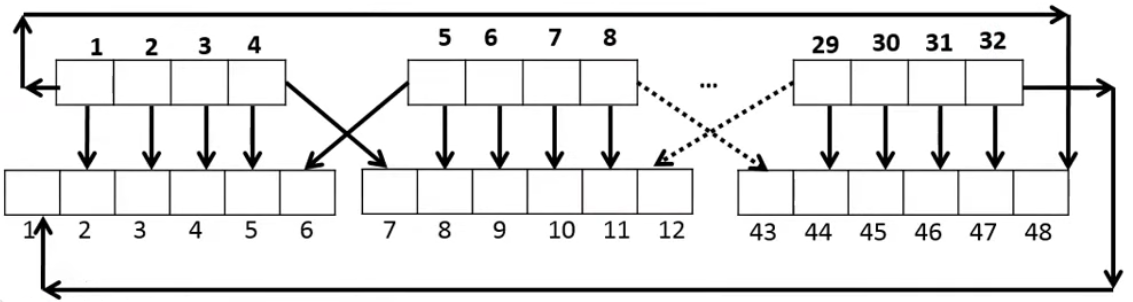
\includegraphics[width=300px]{assets/desExpansion.png}
					\centering
					\caption{Des expansion visulization}
				\end{figure}
				\begin{figure}[h!]
					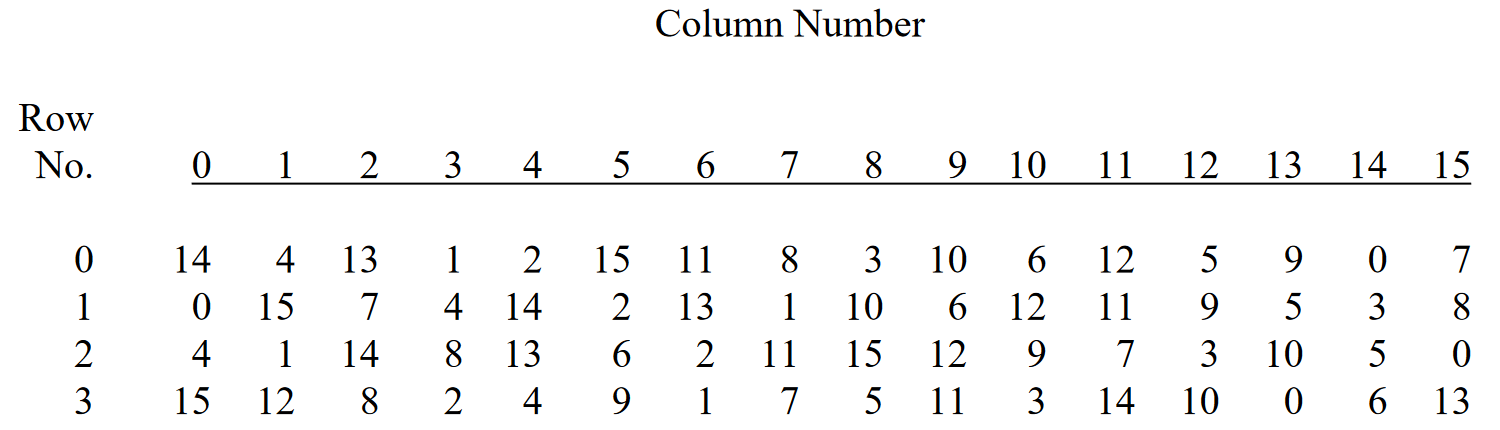
\includegraphics[width=300px]{assets/desSBoxTable.png}
					\hspace{10px}
					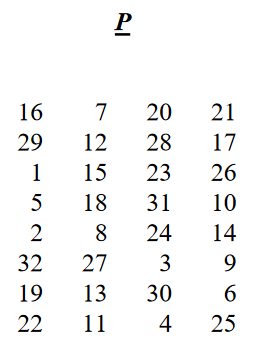
\includegraphics[width=60px]{assets/desPBoxTable.png}
					\centering
					\caption{Des S-Box lookup table to the left and P-box table to the right}
				\end{figure}
				\begin{figure}[h!]
					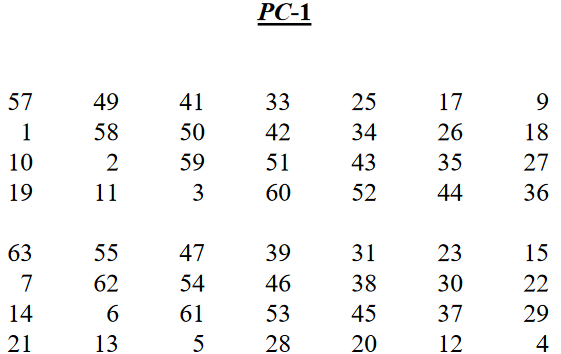
\includegraphics[width=150px]{assets/desPC1.png}
					\hspace{50px}
					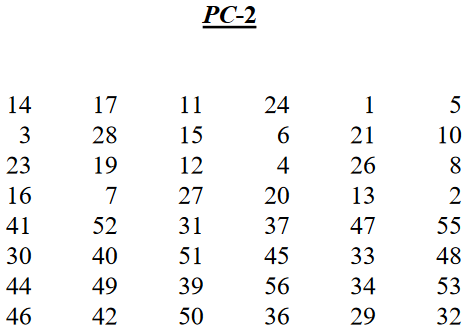
\includegraphics[width=140px]{assets/desPC2.png}
					\centering
					\caption{Des permutation choice tables for creating sub keys}
				\end{figure}
			\subsubsection{Triple DES}
				To get a longer key 3 DES algorithms can be chained.\\
				The encrypt it is done by the three keys $k1,k2,k3$ such ciphertext$=E_{k3}(D_{k2}(E_{k1}(\text{plaintext})))$\\
				For the decryption the encrypt and decrypt is reversed.\\
				The chaining of encrypt decrypt encrypt, is such if a program only implements DES then the triple DES will still work.\\
				Triple is required over double due to double being vulnarable to a meet in the middle attack.\\
				If an attacker has access to the input and output of encryption and decryption and knowns a pair lets say A$\rightarrow$B\\
				Then a DES bruteforce is done with A as input and all outputs are saved. Then B is bruteforce decrypted and all output are saved.\\
				Then a matching pair can be found. This therefore result in two bruteforce has to be done on DES therefore only making the combinations $2^{57}$ and not $2^{112}$
			\subsubsection{AES}
				Plain text is split up into chunks of 128 bits.\\
				There is 3 levels of encryption where 
				\begin{enumerate}
					\item key: 128 bits, rounds: 10
					\item key: 192 bits, rounds: 12
					\item key: 256 bits, round 14
				\end{enumerate}
				The aglorithm works by representing the input as a 4x4 matrix of bytes where the matrix is filled in by columns such b2 is in row 1 column 0, in the following steps
				\begin{enumerate}
					\item Plaintext is XOR'ed with key 0
					\item Sub-bytes - A S-box lookup table is used for substituting bytes
					\item Shift rows - Each row is cyclic left shifted (in bytes) x times where x is equal to the row number 
					\item A mix column matrix is multipled to each column of the matrix
					\item The round key is XOR'ed to the matrix
				\end{enumerate}
				Step 2-5 is repeated, until last round where step 4 is not performed.\\
				To decrypt the keys order is reversed.\\[4mm]
				To find the round keys first a key is generated equal to 128/192/256 bits.\\
				For the 128 bits key
				These are then divided into 4 words of 32 bits denoted $w_i$\\
				Therefore making $k_0=[w_0,w_1,w_2,w_3]$\\
				We can here denote $k_{0-1}=w_1$\\
				To find round $i$'s key the following is done
				\begin{itemize}
					\item $k_{(i-1) - 3}$ is left cyclic shifted
					\item Then it is substituted using the same S-box for the algorithm
					\item Then the round constant is XOR'ed
					\item This is then XOR'ed with $k_{(i-1)-0}$ and is equal to $k_{i-0}$
					\item To find $k_{i-1}$ $k_{(i-1)-1}$ XOR'ed with $k_{(i)-0}$ 
					\item To find $k_{i-2}$ $k_{(i-1)-2}$ XOR'ed with $k_{(i)-1}$ 
					\item To find $k_{i-3}$ $k_{(i-1)-3}$ XOR'ed with $k_{(i)-2}$ 
				\end{itemize}
				The round constants are as follows
		\subsection{Cryptographic hash functions}
			To ensure the integredity of a message a checksum is used.\\
			The is done by the message being sent into a hash function which generates a unique value for the message.\\
			To ensure authenticity of a message, not only is the messaged hashed but a shared key is added to the message. Called message authentication code (MAC)\\
			Then when the message is received the message is also hashed and checked to be equal to the sent hash value.\\
			This shared key could then be shared using RSA.\\[4mm]
			To get a digital signature the private key can be used to encrypt a document which then people can verify by decrypting using the public key.\\
			This can then be combined with the MAC, such a method can both have integrity and verified arthour. After generating the hash the senders private key is used to encrypt the hash, which then can be decrypted and verified.\\
			A certification authory (CA) is used to hold public keys and verify to whom a public key belong to.\\
			An authentication protocol can work by first teh sender sends an initiating message, the receiver response with a nonce (never used number), the sender encrypts using private key and receiver decrypts using public key. If they match an uthentication is established.\\
		
		\subsection{Diffie Hellman key exhange}
			Allows two parties that have no prior knowledge of each other tojointly establish a shared secret key over an insecure channel.\\
			The exhange is based on:
			\begin{enumerate}
				\item A common ground such as a number
				\item Client and server adds their own number to the common ground
				\item Client and server switch keys
				\item Client and server again adds their own number
				\item Client and server now has the same number
			\end{enumerate}
	\section{Transport layer}
		The transport layer is the messenger between the network layer and applicaiton layer.\\
		Therefore the transport layer is only at presense in the end systems of the network.\\
		The transport layer provides protocols for UDP (User datagram protocol) and TCP (Transmission control protocol)\\
		Transport layer packet is called a segment.\\
		The IP is an unreliable service which does not guarantee segment delivery, in order and integreity\\
		This is therefore encounted for in the transport layer.\\
		\subsection{Multiplexing and demultiplexing}
			Demultiplexing is when a segment redirects a data to the correct socket.\\
			Multiplexing is creating segments with header information for the demultiplexing.\\
			The segment header therefor has two fields of 16 bits the source port and detination port.\\
			The well-known port numbers are from 0 - 1023 and are restricted, for things like HTTP and FTP\\
			In case of a server setup with TCP, the server then uses the four parameters in the TCP request (src ip, dest ip, src port, dest port) to setup a demultiplexing on a new port.\\
			Such two client may connect to the same port and unknowingly be switched to a new port without having to change TCP parameters.
		\subsection{Reliable data transfer}
			To verify (positive aknowledgments) or request repear (negative acknowledgment) data transmission is known as ARQ (Automatic Repaeat reQuest) protocols\\
			An ARQ protocol requires error detection, receiver feedback and retransmission\\
			This type of protocol will only send new data when the receiver aknowledge the package was received, therefore the name stop-and-wait protocols.\\
			The problem is if the aknowledgment is corrupted, to counteract this the package is sent with a sequence number and in case of unidentifiable aknowledgment the packet can be sent again.\\
			Likewise the acknowledgment also gets the sequence number to counter act dublicate acknowledgments.\\
			The sequence is simply a single bit, to know that the packet is in the right order relative to the last packet.\\
			In case of a lost package or aknowledgment the sender has a time of which after it will resend the package\\
			Choosing the time is hard and must be estimated to be fast enough to not wait too long but still not send too many dublicate packages.\\
			Pipelining is the act of sending multiple packages at once, and increasing the sequence numbering.
			\subsubsection{Go-Back-N}
				GBN is a protol which allows the sender to send $n$ packages at once.\\
				To protocol states that the base is the sequence number which is next to be aknowledged\\
				The nextseqnum is the next package to be sequenced and sent.\\
				The protocol can also be called sliding-window protocol because it can be seen as a windows swhich slides over the packages to send.\\
				GBN only use a single timer for all package refering to the last not aknowledged package. If the time runs out all non aknowledged packages are resend.\\
				If the receiver get an out of order package the package is discarded and a negative aknowledgment is sent, where the sender will resend all non aknowledged packages.\\
				Selective repeat combats this by only sending negative aknowledged or timeout packages from which the receiver must keep a buffer of correct and always aknowledge good packages.\\
		\subsection{TCP}
			TCP is duplex thus allowing data in both directions at once.\\
			TCP is a hybrud if selective repeat and Go-Back-N\\
			TCP is point-to-point at therefore only two host can be part of a TCP connection\\
			First a three way handshake is made with no payloads.\\
			Then a send buffer is initialized and the application fills it up.\\
			Then the TCP chooses when the create a segment with buffer data.\\
			The maximum segment size (MSS) is determiend maximym transmission unit (MTU) (1500 bytes in ethernet and PPP) minus header data from IP and TCP (typically 40 bytes) \\
			The segment header includes the same as UDPs (src, destination port number, checksum)
			\begin{itemize}
				\item 32 bit sequence field
				\item 32 bit sequence aknowledgment field
				\item Receive window indicating number of bytes receiver is willing to accept
				\item 4 bit header length field representing number of 32 bit header lengths
				\item Optional field include timestamp, agreed MMS, windows scaling factor 
				\item 6 bit flag field: 
				\begin{itemize}
					\item ACK bit for aknowledgement 
					\item RST, SYN, and FIN for connection setup and teardown
					\item CWR and ECE for congestion notification
					\item PSH pass data to upperlayer immediately
					\item URG for urgent segments
				\end{itemize}
			\end{itemize} 
			\subsubsection{Sequence numbering}
				The TCP sequence numbering is on every byte and the segments numbering is the first bytes number.\\
				Aknowledge numbering works by the response is the next expected aknowledge number. \\
				Say the host recieves a packet segment 0, length 447 bytes, then the host responds with aknowledge number 448\\
				TCP is therefore said to provide commulative acknowledments.\\
				In case of out of order packages the individual implementation decide to either buffer it or discard it.
			\subsubsection{Timeout time}
				To find segment timeout the first the round trip time (RTT) is calculated using the formula
				$$\text{EstimatedRTT}=(1-\alpha)\cdot \text{EstimatedRTT}+\alpha \cdot \text{SampleRTT}$$
				Where $\alpha=1/8$ and it can be noted that the new sample is more weighted.\\
				The variation is also important and is calculated using
				$$\text{DevRTT}=(1-\beta)\cdot \text{DevRTT}+\beta \cdot |\text{SampleRTT}-\text{EstimatedRTT}|$$
				Where the recommeded value is $\beta = 0.25$\\
				The timeout is then determined as
				$$\text{TimeoutInterval}=\text{EstimatedRTT}+4\cdot\text{DevRTT}$$
				For the first package it is set to 1 second and when a timeout occurs the value is doubled.
				When measuring only orginal packages are measured such a false time is not measured from a newly sent and old aknowledgment\\[4mm]
				Fast retransmit can occur if a triple duplicate aknowledge is gotten. Three is choosen since a double could accour in the event of out of order, but three will most likely be a missing segment.\\
				Then the timer is ignored and the second is sent as soon as possible.
			\subsubsection{Flow control}
				Flow control is used in case the application is reading data slower than TCP is receiving the therefore overflowing the receiver buffer.\\
				The receiver buffer spare room called receive window will always be equal to 
				$$\text{rwnd}=\text{RcvBuffer}-\text{LastByteRcvd}-\text{LastByteRead}$$
				Where LastByteRead is the byte numbering read by the application.\\
				Therefore the sender will not send more bytes than LastSendByte-LastAckedByte\\
				When the rwnd is 0 the sender have to send bytes until acknowledgment and a non zero rwnd is sent by the receiver
			\subsubsection{Connection management}
				A TCP connection is established by
				\begin{enumerate}
					\item A segment without application data is sent with SYN flag set to 1 and a random segment number
					\item The server allocates space for variables and buffer and send a segment with SYN = 1, ACK = segment number +1 and a segment number the server itself chooses randomly
					\item The client allocates space for variables and buffer and sendst the first data with ACK = server segment number +1 and SYN = 0
				\end{enumerate}
				When a TCP connection is shutdown the following is done
				\begin{enumerate}
					\item Client send a segment with FIN flag = 1
					\item Server acknowledges the FIN flag
					\item Server sendt a segment with FIN flag = 1
					\item Client achknowledges the FIN flag 
				\end{enumerate}
				When the last step is done 30 seconds is waited before closing fully down.\\
				When TCP acknowledges a FIN segment the variables and buffer space deallocated.\\
				The TCP from client has 6 stages
				\begin{itemize}	
					\item SYN\_SENT - Send SYN
					\item ESTABLISHED - Receive SYN \& ACK, send ACK
					\item FIN\_WAIT\_1 - Send Fin
					\item FIN\_WAIT\_2 - Receiver ACK
					\item TIME\_WAIT - Receive FIN, send ACK
					\item CLOSED - Wait 30 seconds
				\end{itemize}
				The TCP for server has 6 stages
				\begin{itemize}
					\item Listen - new open socket
					\item SYN\_RCVD - Receive SYN, send SYN \& ACK
					\item ESTABLISHED - Receive ACK
					\item CLOSE\_WAIT - Receive FIN, send ACK
					\item LAST\_ACK - Send FIN
					\item CLOSED - Receive ACK
				\end{itemize}
				
				In the case of the server receiving a TCP request on a non TCP port a segment with RST flag is sent back.\\
				For a server to prevent SYN flooding, a hash of the client is made from IP, sorce and port number called cookie and is sent as segment numbering and forgotten.\\
				When receiving the SYNACK the cookie is recalculated and only if the ack is cookie +1 will the server allocate space and recognize it as a legitimate request.\\
			\subsubsection{Congestion Control}
				Classic TCP uses end-to-end congestion control rather than network assisted (Where router indicates to host if congestion is a problem).\\
				To exercise congestion control the sending rate is limited to
				$$\text{LastByteSent} - \text{LastByteAcked} \leq min(\text{cwnd},\text{rwnd})$$
				Where cwnd is congestion window.\\
				cwnd is determined by
				\begin{itemize}
					\item If a timeout occours or a retransmission the cwnd is lowered
					\item A successfull delivery will increase the cwnd
				\end{itemize}
				The algorithm therefore works by first starting in slow start with cwnd = 1 and is knwon as additive-increase,multiplicative-decrease (AIMD)
				\begin{itemize}
					\item Slow start - First the rate is 1 MSS, then for every acknowledged segment 1 MSS is added to cwnd essentially doubling it until a problem occour. When that happends a variable ssthresh is initiated to cwnd/2 and cwnd is set to 1. Then again slow start is begun on it until it reaches sshtresh from which congestion avoidance is begun. In case of 3 dublicates fast receovery is ran with ssthresh = cwnd/2 and cwnd = sshtresh + 3MSS
					\item Congestion avoidance - Now cwnd is incremented only by MSS/cwnd until a problem occour. If a dublicate occour three times sshtresh is updated to cwnd/2, cwnd is set to ssthresh + 3 MSS and fast recovery is ran. If a timeout occurs sshtresh is set to cwnd/2 and cwnd is set to 1.
					\item Fast recovery - cwnd is incremeneted by a single MSS. In a timeout sshtresh = cwnd/2, cwnd=1 and slow start is begun.
				\end{itemize}
				The Cubic version is an alternative where the congestion avoidance saves the last max limit it reached and then cubicly reaches it such the farther the distance to the maximum the more cwnd is increased.\\[4mm]
				The network assisted version works by, the router sets the ECN (Explicit congestion notification echo) flag on a segment to the receiver, which also sets it in the acknowledgment. Which result in hafling the congestion window\\
				Delay based congestion control works by using the RTT, if the sender then measures a significantly less tha nthe uncongested througput rate, then it slows down the sending rate. Essentially it works by avoiding queues.\\[4mm]
				It can be seen TCP will fairly share bandwith and conestion controle will be equal in multiple TCP connections over time.\\
				This is unlike UDP which will not behave fair and force TCP to get less bandwith without itself taking less.
		\subsection{QUIC}
			QUIC is an extension to the UDP protocol, which provides features from TCP.\\
			A handshake is initiated, but it only needs a single send and receive to setup therefore saving a whole RTT over TCP.\\
			Even QUIC-0 can be used in case of recent connection where no handshake is needed as saved params are used.\\
			QUIC provides encryption of packages and uses http3.\\
			QUIC uses reliable, and congestion controlled data transfer features from TCP
		\subsection{TLS}
			Transport Layer Security (TLS) is an extension to TCP which gives it security in the form of: encryption, integreity and authentication.\\
			Websites using TLS is recognized by the use of https.\\
			TLS acts as a sublayer in the TLS socket and applies it security.\\
			When running TLS the data is split up into records which is encrypted and hashed using HMAC.\\
			The TLS record consist of: Type, Version, Length, Data, and HMAC, where data and HMAC is encrypted with $E_B$\\
			The type field is used for a copy of the TCP type, such as FIN flags but by using it in the TLS, it is included in the hashing such no tampering of the TCP flags will destroy the connection.\\
			Likewise is the sequence numbe and length of message also part of the hash .\\
			A TLS connection is as follows:
			\begin{enumerate}
				\item A list of supported cryptographic algos and a nonce is sent from client
				\item Server chooses a cryptographic alg. for symmetric key, public key and hmac. Then responds with choices, certificate and server nonce
				\item Client confirms certifcate and gets server public key, generates Pre-Master Secret (PMS), and sends encrypted PMS with server public key
				\item Using the choosen algos the server and client generates Master Secret (MS) from PMS and nonce. The MS is sliced up into: 2 encryption keys, 2 HMAC keys, initialization vectors in case of symmetric cipher
				\item Client send HMAC of all handshake messages
				\item Server send HMAC of all handskake messages
			\end{enumerate}
			The HMAC handshake messages are used to ensure integrety of the non encrypted handshakes before. Likewise is the nonce used to prevent replay attacks. \\
			The keys generated from the MS is denoted
			\begin{itemize}
				\item $E_B$ session encrypted key for data from client to server
				\item $M_B$ session HMAC key for data from client to server
				\item $E_A$ session encryption key for data from server to client
				\item $M_A$ sessuin HMAC key for data from server to client
			\end{itemize}
	\section{OWASP - Top ten seciruty risk}
		Open Web Application Security Project conducted a list of biggest security risk based on data on attacks. The following the that top then in order. 
		\subsection{Broken Access Control}
			The biggest problem is allowing attacker acces to data or controle which was not intended.\\
			This may be can be through websites, API or any other access to data or controle.\\
			Problem often occur due to amount of access points and lack of testing.\\
			Attackers often use modification of accessible data, such as cookies or url which may not be sanitized.
		\subsection{Cyptographic Failues}
			Many systems and companies may use old cryptography or non at all on sensitive data.\\
			This can also be in form of transportion of data both internal and external.\\
			Lack of this will result in case of leaks actually exposed data rather than encrypted data.
		\subsection{Injection}
			Injections occur when user data is sent to an interpreter without sanitizing the input.\\
			The can be queries for databases or bad designs for inputs which can result in bad input.\\
			This can be in buffer overflows which may allow injection of code and gaining access to higher priveledge.\\
		\subsection{Insecure Design}
			Insecure design is not the implementation but rather the security choices.\\
			This can be password recoveries which is too weak or intern protocols which may be too weak when handlign sensitive data
		\subsection{Security misconfiguration}
			This may be outdated libraries or default setting which is unchanged and therefore leaves a vulnarability.\\
			This may also be in case of settings for development end up in production leaving a open backdoor or like wise.
		\subsection{Vulnarable and outdated components}
			Likewise seciruty misconfiguration but this focus more on the oudated packages or libraries which may be in use.\\
			The libraries may contain vulnerabilities which can gain acces to the code or data.\\
			This is prevented by subscribing to bulletins of included libraries or packages and keeping them up to date.
		\subsection{Identification and authentication failues}
			Bad implementation of authentication which gives attackers opportunities to gain access via session tokens, keys or passwords.\\
			This can be in the form of, allowing brute force attacks, allowing weak passwords or having a weak password recovery\\
			A good solution is often implementing two step authentication.
		\subsection{ Software and data integrity failues}
			This happends when an attacker identifies as software or plugin and forces an update upon working code.\\
			This may also be if an attacker simply notices a data stream which does not check for integrety and themselves may send attacking data.
		\subsection{Security logging and monitoring failures}
			Most attacks are not detected before 200 days after.\\
			This is due to lack of securty logging and monitoring attacking attemps.\\
			A better monitor or log may capture attemps and warn of risky areas before an attack happen
		\subsection{Server side request forgery}
			When a web application is fetching remote ressource without validation.\\
			This may lead to an attacker beign able to load attack ressources onto the application.\\
			This is prevented having a firewall which block all trafic beside the known remote places.\\
	\section{Penetration testing}
		The two most comon forms of penetration tests are:
		Application penetrations testing and infrastructure penetration testing.\\
		Other types are
		\begin{itemize}
			\item Mobile application
			\item Device penetration testing (laptops, consumer devices)
			\item Wireless penetration testing
			\item Telephony or VoIP 
		\end{itemize}
		There are three different types of intruders
		\begin{itemize}
			\item Hackers - Experimentally minded programmers targets security loopholes in it system
			\item Crackers - Exploits weak points of it systems to gain illegal advantages
			\item Insiders - Type of crackers with inside knowledge
			\item Script kiddies - Uses attack tools
		\end{itemize}
		There are mainly 3 different types of attacks
		\begin{itemize}
			\item Network based attacks - attacks using network protocol functionalities this includes port scanning, IP spoofing, sniffing, session hijacking, DoS attacks, buffer overflow and format string attacks
			\item Social engineering - Maniupulating people to revela security related information 
			\item Circumventing of physical security measures - By using physical attacks and gaining access to physcial data or authority
		\end{itemize}
		A company should have secuirty policies and secuirty concepts, without that a pen test would not even be helpfull.\\
		The procedure of pen testing are in the following steps
		\begin{enumerate}
			\item Research information about the target system - information like official IP address
			\item Scan target systems for service on offer - Using a port scan internet services can be found
			\item Identify systems and applications - By using fingerprints in the prt scan
			\item Research vulnerabilities - Finding exploits in systems with open ports from fingerprints
			\item Exploirt vulnarabilities - Using the known vulnerabilities and gaining access for further attacks
		\end{enumerate}
		\subsection{Classifying pen tests}
			Starting point - Attack of penetration most common: firewalls, web servers, RAS access points and wireless networks.\\
			External servers are known as normal workstations.\\
			Web serbers are often vulnarable due to there minufold of functions\\
			Pen testing is usefull since security audits and IT audits most often focus in IT infrastucture in terms of compliance, efficiency nad efectivness.\\
			The goals of pen testing should be clear and can be divided into four categories\\
			\begin{itemize}
				\item Improving security of techinal systems - This can be finding improvements in firewalls, routers, web servers, etc..
				\item Identifying vulnarabilities - This is the actual objective of the test
				\item Having IT security confirmed by an external third party - The IT system and infrastructures current security
				\item Improving security of orginazational and personnel infrastructure - This is often in form of social engineering
			\end{itemize}
			The limtis of a pen test is the fast discovery of new vulnarabillities making pen test only validation of security currently but not in the future.\\
			Likewise does the pen test reduce the probabillity of a successfull attack.\\
			The type of attack is also classified to test a given scenario\\
			\begin{figure}[h!]
				\centering
				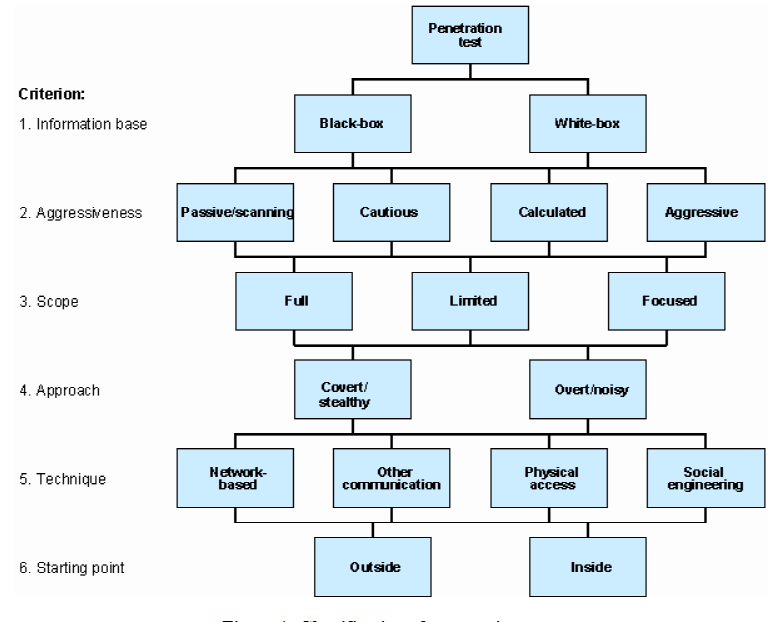
\includegraphics[width=300px]{assets/penClassification.png}
			\end{figure}
			\begin{itemize}
				\item Information base - The amount of known information, where black box represent the unknown insider information unlike white box
				\item Aggressiveness
				\begin{itemize}
					\item Passively - Vulnerabilities are detected but not exploited
					\item Cautious - Vulnarabilites are only tested when it will not result in system suffering
					\item Calculated - Exploits vulnarabilities which may result in system disruptions
					\item Aggressive - Exploit every vulnarability even if deactivating systems or overloading
				\end{itemize}
				\item Scope - The amount of testing which directly relates to time spent, focused sub network after modifcation, limited number of systems, full everything avaliable
				\item Approach - How visible the attack is, covert stealthy, overt often with staff such fixes can fast be done
				\item Technique - Networks based using network protocols also known as IP-based pen test, Other communcation networks, mobile, fax, wireless networks etc., physical in case of good enough firewall, social engineering people are frequently the weakest link
				\item Starting point - Is the test performed from an outside perspective, or inside networks where firewalls do not have to be overcome
			\end{itemize}
			Most often a combination of pen tests are adviceable.
		\subsection{Legallity and ethical issues}
			There are different legal issues which rises from pen testing.\\
			For a company pen testing may be needed, to ensure data security to compart with laws.\\
			When a pen test is performed approval by client in all areas is required.\\
			Likewise often 3rd oarty also need to approve the test\\
			The test should have a liability to cover claims from 3rd parties.\\
			Ethical issues also araise with social enginering in case of wanted anonymity.	
		\subsection{Phases of pen testing}
			\begin{figure}[h!]
				\centering
				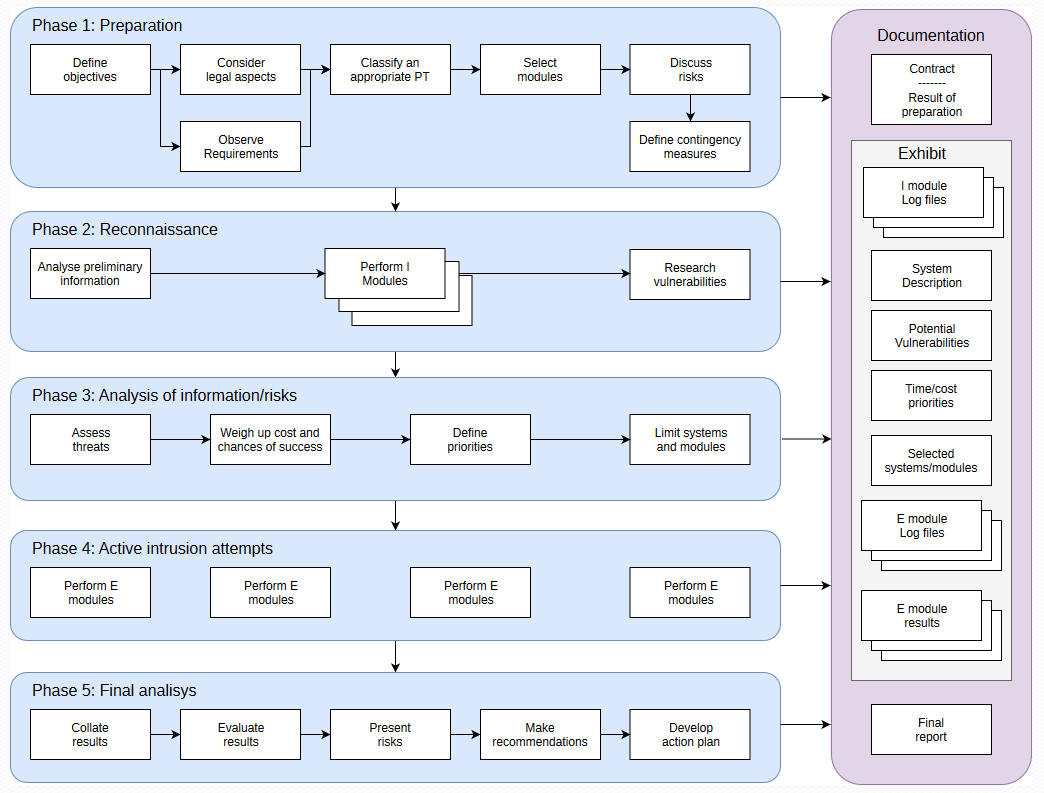
\includegraphics[width=300px]{assets/penPhases.png}
			\end{figure}
			Preparation - agree on scrope and cost based on classification, contracts in plase and discuss risks\\
			Reconnaissance - passive test, where information is obtained and overview of system.\\
			Tool for data collection
			\begin{itemize}
				\item whois
				\item https://website.informer.com/
				\item namp 
				\item https://spokeo.com/
				\item osint examples 
				\begin{itemize}
					\item https://www.shodan.io/
					\item https://www.spiderfoot.net/
					\item https://github.com/laramies/theHarvester
				\end{itemize}
			\end{itemize}
			Analyzing infromation and risks - use data to find risk and determine which to test based on goals and time\\
			Active intrusion attempt - This phase test the vulnarabillities found, it is here important to consider actual risks and whihc risk are not affecting the product/organization\\
			Final analysis - Evaluate the vulnarabilities and where they where found and recommandation to eliminate them\\
		\subsection{Tools}
			\begin{itemize}
				\item Kali linux - OS with preinstalled tools
				\item Nmap - port scanning
				\item NCAT - Read/ write network connection using TCP or UDP
				\item Metasploit - Frameowrk woth most common exploits
				\item SQLmap - Detecting and xploiting sQL injections flaws
				\item NIKTO - Scan for harmful files, misconfigurations, outdated software installations on web server
				\item BURPSUITE - Pen testing web application tool
				\item John the riper - Tool for cracking password
				\item NESSUS - vulnerability scanner (not free)
				\item Wireshark - Packet sniffer and network analyzer tool
				\item AIRCRACK-NG - wireless network tool
				\item Tool list - https://sectools.org/
			\end{itemize}
	\section{The network layer: Data plane}
		The role of the network layer is the route packets from host to receiver.\\
		Routing is done by the all routers by each forwarding the packet from input to correct output link.\\
		This is done using routing algorithms.\\
		The result of routing algorithms is a forwarding table which determines which output link the router should forward to.\\
		There are two approaches to creating the forwarding table either the routers share their tables between eachother using a routing protocol.\\
		Or the SDN approach where an external remote controller creates tables for routers and send them it. This can be done by third parties or ISP.\\
		SDN stands for software-defined networking.\\
		The networks service model is defined to be best-effort service therefore many features are not implemented other than trying to deliver.
		\subsection{What is insde a router}
			Input ports is used for terminatign incomming physical link.\\
			The input performs the lookup function to the forward table via the switching fabric.\\
			In case of a control packet the packet is forwarded to the routing processor.\\
			The switching fabroc connects the input and output ports.\\
			The putput ports store the sending packets and perform the necessary link-layer and physical layer functions.\\
			THe routing processor maintains the router, by updating the forwarding tables or in case of SDN connects to remote and update forward tables.\\
			The forwarding tables matches a prefix of the packets destination address.\\
			If a match does not exist it exists via the default port.\\
			If multiple matches the longest is choosen.\\
			If the ports is in use the fabric blocks the package and queues it.\\
			All this has to happend in hardware to keep up with transfer speeds.\\
			The input port also has to, physical and link layer processing, check the checksum and time to live, update counters and time to live.\\
			\subsubsection{Switching}
				The act of switching can be done through different methods.\\
				The simplest version switching via memory, copies inputs into processor memory and let the processor due to moving to output.\\
				This is limited to memory bandwidth and therefore the transfer will be limited to half the memory bandwaidth.\\
				Switching via a bus transfers packets via a bus, then every packet get appended a label and the matching output port keeps the packet the rest throws it away.\\
				The label is then removed before sending.\\
				This is then limited to the bus speed since only one package can be worked with at a time.\\
				Switching via an interconnection network, uses a crossbar switch, where a bus from every input goes over output ports bus, such an intersect is present for each.\\
				Then the intersect between input and output is turned on to forward the package.\\
				This results in the package only being blocked in case of the wanted output is taken.\\
				More sophisticated approached uses a stacked interconnect such the output can contain multiple packages
			\subsubsection{Queue and buffers}
				Queue can occuor both on output and input, input will happen when either too many packages comes into one input at once or head of the line (HOL) blocking, where another input waits for output and therefore block the input buffers.\\
				Output will occur if the transmission rate is slower than the forwarding and input.\\
				When queue occuor either the latest (drop tail) is dropped or a random picked using an active queue management algorithm\\
				The drop tail has the advantage of faster congestion signalling to sender.\\
				The size of the buffer has to be large enough to prevent package lost too fast in case of a burst, but smaller than queuing delays are too high.\\
				The rule of thumb is a buffer size equal to 
				$$B=RTT\cdot C/\sqrt{N}$$
				Where $C$ iis the link capacity and $N$ is the number of independent TCP flows.\\
				TCP is part of the equation since in case of a buffer being filled up, since TCP will recieve an ACK for every sent from the buffer the buffer will never empty known as bufferbloat.\\
				For emptying the queues different approaches can be taken
				\begin{itemize}
					\item First in first out FIFO - The packages is handled in the same order as arrival
					\item Priority queuing - The packages are classified upon arrival which then is handled in priority order
					\item Round Robing and Weighted fair queung - Like priority queuing, but to ensure every package is sent at some point the queues is served in a circular manner. The class weight then determines the time used pr. queue such higher priority equals more time spent in the queue before moving on.
				\end{itemize}
		\subsection{The interprotocol (IP)}
			\subsubsection{IPv4}
				The datagram of an IPv4 is
				\begin{itemize}
					\item Version number - 4 bits to determine version number like IPv6
					\item Header length - IPv4 datagram contains variable headers therefore 4 bits is used for indicating size
					\item Type of service - Used to distinguish if the package is a real-time datagram or an non-real-time traffic like FTP, in here two bits are also used for congestion control
					\item Identifier, flags, fragmentation offset - Used for IP fragmentation 
					\item Time-to-live - Counter for number of routers which the package can be sent through before being dropped
					\item Protocol - A number representing which protocol is used after the IP the handle the data like TCP or UDP
					\item Header checksum - Checksum of the integer value of every second header values sum. Recalculated for each router step since headers changes like time to live
					\item Source and destintion IP
					\item Options - Allow to extend the IP headers further
					\item Data
				\end{itemize}
				The header is 20 bytes without options and with IP the size is 40 bytes\\
				An interface is the boundary between link and host and has each their own IP.\\
				With a 32 bit long IPv4 the total number of IPs is $2^{32}$ or aprox 4 billion\\
				The IP is formatted into 4 chunks bytes which is written in decimal with dots between the decimals.\\
				Subnets can be defined such a prefix is the identifier and then the whole subnet uses the prefix and the rest is for intern routing.\\
				This is in the format a.b.c.d/x where x is the number of bits used for the prefix and the rest is the subnet.\\
				This is known as Classless interdomain routing (CIDR). This allows for subnets to have way smaller forwarding tables.\\
				Before CIDR the subnets size was bounded to 8, 16 or 24 bits making the jump from 8 to 16 very large.\\
				255.255.255.255 is used for sending a package to every device in the subnet.\\
				To get a subnet the isp is contacted which will give part of their subnet to the company.\\
				The isp subnet is managed by regionals which is managed by Internet corporation for assigned names and numbers (ICANN).\\
				ICANN is a NPO which mangages DNS root servers, assigning fmain names and resovlg=ving dfomain name disputes.\\ 
			\subsubsection{Obtaining an address}
				Dynamic Host Configuration Protocol DHCP is a protocol used to configure devices by admins.\\
				DHCP allows to assign a static IP to devices or temporary IP.\\
				DHCP requires a server or device which reulays the DHCP protocol.\\
				The protocol consist of
				\begin{itemize}
					\item DHCP server discovery, which is an udp packet send to port 67 to 255.255.255
					\item DHCP server offer(s) - Once a discovery is gotten a offer is sent back to the subnetwork, and contains transaction ID, proposed IP, network mask and IP address lease time (The time the ip is valid)
					\item DHCP request - Client chooses from offers and respond to the wanted by echoing the content
					\item DHCP ACK - an acknowledment message is sent confirming the device
				\end{itemize}
				The problem with DHCP is the requirement for the protocol for every subnet which is a problem in case of more routers in large areas.
			\subsubsection{Network address transaltion (NAT)}
				NAT is a method for using a routers as a single device.\\
				This allows for a single IP which is shared among the local network.\\
				This works by when a device sent a package to the router, the request is contains the wanted IP and a socket to the device from route.\\
				The router then rewrites the source and source ip to the wan ip.\\
				This allows up to 60,000 devices on one network with 1 ip address.\\
				This is argued against since is reuses port numbers for addressing purposes.\\
				This also requires for server like application a NAT traversal tool for finding open ports in the local network.\\
				ANother problem is it ruins the archtiecture of the internet, by not assigning devices an IP but rather a number of devices.\\
			\subsubsection{IPv6}
				The problem with IPv4 is the limited amount of IPs.\\
				The last IPv4 address space was given out in 2011 to a reginal registry.\\
				There is open IPv4 address in regionals but the global pool is empty.\\
				IPv6 uses 128 bits to create IPs making sure it will never be problem again.\\
				The format goes as
				\begin{itemize}
					\item Expanded addressing capabilities - This allows to send a package to an IP group 
					\item A streamlined 40 byte header 
					\item Version - nubmerical value 4 for IPv4 and 6 for IPv6
					\item Traffic class - 8 bit field for priority certain diagrams
					\item Flow label - Allowing to label packages as flow and given them optional priority
					\item Next header - Like to protocol in IPv4
					\item Hop limit - Like time-to-live in IPv4
					\item Source and destination addresses
					\item Data
				\end{itemize}
			\subsubsection{Openflow}
				Openflow is the mechanism which performs the match and action for packages.\\
				The mathc is done over the whole datagram, including link,- network,- and transport layer.\\
				The there means\\
				\begin{tabular}{|c|c|c|c|c||}
				\hline
				Ingress port &&&&\\
				\hline
				src MAC & dst MAC & eth Type & VLAN ID & VLAND Pri \\
				\hline
				IP src & IP dst &&&\\
				\hline
				IP proto & IP TOS & TCP/UDP src port & TCU/UDP dst port&\\
				\hline
				\end{tabular}
				From this a flow table is generated which states rules, and matching will be used in priority order.\\
				Each row then has a list of action which in done in the given order.\\
				The include forwarding, dropping and modifying fields.\\
				This can be used to create firewalls by blocking IP or methods by dropping the matching columns
			\subsubsection{Fragmentation}
				The fragmentation of a packet is the act of splitting up the package such they can fit into the maximum transfer unit (MTU)\\
				The header will have offset set such the packets order can be seen and is divided by 8 bytes to save space.\\
				The offset will come from the previous packages data length (not inclduding header 20 bytes if no options)\\
				The fragflag is not raised on the final package. \\
				The fragflag is raised and the ID will match across the framentations.\\
	\section{Control plane}
		\subsection{Routing algorithms}
			Routing algorithms is used to find the least cost routes between sender and receiver.\\
			The cost may reflect, physical length, speed or mentary cost of links.\\
			Two nodes cost is said to be $c(x,y)$ and in case of not being connected the cost is infinite.\\
			The graphs is considered undirected.\\
			Centralize routing algorithmms use global knowledge of the network.\\
			To communicate a link-state broadcase algorithm is used. From this the Dijkstras aglorithm can be used to find least cost to each node.\\[4mm]
			The algorithm will run at a centralized unit and the algorithms is refered to as link-state (LS) algorithm\\
			Decentralized rounting uses iterative, distributed manner by the routers.\\
			The routers only have knowledge of neightbour routes and the cost to them.\\
			The routers then exhange information about their neightbours to calculate the cost further.\\
			This is called distance-vector (DV) algorithm.\\
			This is done async by to nodes does need to work at same time, and iterative by how each nodes send and updates on changes.\\
			The network cost is then calculated using bellman-fords algorithm.\\[4mm]
			Algorithms can also be classifed by being static which change slowly over time.\\
			And dynamic which changes for every traffic loads or topology change.\\
			Load sensitive algorithms takes the package load into account to congestion.\\
			\subsubsection{Problems}
				Oscillations is where a network of nodes oscillates between two optimal path and therefore never end termination.\\
				To prevent this the routers send their link advertisment at random intervals to also prevent self-synchronizing.\\
				Count to infinity problem occur if the nodes A,B and C is connected with cost 1.\\
				If B and C is disconnected and does not send an update before A sends an update to B and advertise its length to C at 2.\\
				This will then result in B updating to 2, A updating to 3 since it used B to get to C. This will then keep happening until they count to infinity.\\
				A solution which works with small node envirements is the poisoned reverse, which advertises when routes is broken or increased.
			\subsubsection{BGP}
				BGP is a protocol for connection between AS\\
				In the AS there are two types of routers, gateway routers on the edge connecting between AS and internal.\\
				The BGP protocol uses TCP since it needs to transfer large amount of data, here the forwarding tables in other AS.\\
				The BGP protocol comes in two types iBGP and eBGP\\
				iBGP is for internal use, such when a new forwarding table has come into the AS it is shared between internal routers using iBGP\\
				eBGP is external BGP which communicates between different ASs.\\
				A new external forwarding table may include everything to AS1 goes through routerA.\\
				The internal then simply uses the optimal path to get the a router which is a gateway.\\
				BGP routing is done through different methods
				\begin{itemize}
					\item Hot potato - The AS focuses only on reducing cost internally and ignore outside policies.
					\item Route-selection - This is the used algorithm used in case of multiple routes and the route is selected in the given order
					\begin{itemize}
						\item Check local preferences on attributes which is determined by policies
						\item The shortes AS path is chosen
						\item Hot potato is used
						\item BGP identificers is used to select
					\end{itemize}
				\end{itemize}
				BGP is also used to find the nearest DNS server, using IP-anycast.
			\subsubsection{SDN control plane}
				Software defined network (SDN) network with seperated controller.\\
				A SDN network can be identified by the following characteristics
				\begin{itemize}
					\item Flow based forwarding - Packet forwarding can be don based on any number of header fields
					\item Seperation of data plane and control plane - Instead of the routers doing both data and controle plane, is the control plane done by a seperate entity
					\item Network control functions - Communicate between a SDN controller and network control applications
					\item A programmable network - Using API in the SDN controller the network switches can be programmed
				\end{itemize}
				A SDN controller consist of 
				\begin{itemize}
					\item A communication layer - Communication between SDN controller and controllers using open flow or other protocols
					\item A network-wirde state-management layer - Control decisions, such as flow tables, load balancing or firewalling capability
					\item The interface to the network-control application layer - Interfaces for read/write network state and flow table
				\end{itemize}
				In practise the SDN controller consist of distrubted set of servers for fault tolerance, hight availability and performance.
			\subsubsection{Openflow}
				Openflow uses the TCP protocol over port 6653\\
				Openflow allows for messages from SDN controller to controlled switch 
				\begin{itemize}
					\item Configuration - Set a switch configuration params
					\item Modify-state - Add/delete entries in the flow table
					\item Read-state - Collect statisticts from flow table and ports
					\item Send-packet - Send a packet using the controller
				\end{itemize}
				From the controller switch the SDN controller can get the packages
				\begin{itemize}
					\item Flow-removed - Flow entry on table has been removed
					\item Port-status - Change in ports
					\item Packet-in - Packets wich does not match table or should be sent to controller
				\end{itemize}
	\section{IPsec and VPN}
		IP security protocol (IPsec) is a security protocol applied in network layer on the IP datagrams.\\
		This is what enables virutal private networks (VPNs)\\
		IPsec puts a security layer on top of the payload such as TCP, UDp pr ICMP.\\
		The IPSec can provide, source authentication, data integrity, and replay-attack prevention.\\
		A VPN can be desired in a institution placed in multiple geographical locations.\\
		This will then make is possible to create a secure network conenction between locations over the public network.\\
		IPsec can use two protocols: Authentication Header (AH) and Encapsulation Security Payload (ESP)\\
		They both provide source authentication and data entregrity but ESP provide confiendtialy and therefore is used more.\\
		Security Associations (SA) is a network layer logic connection which is undirectional.\\
		If both entities want to send secure datagrams both has to setup a SA connection.\\
		The SA has attributes which both sender and receiver keep track of
		\begin{itemize}
			\item 32 bit identificer for the SA called security paramete indes (SPI)
			\item Origin interfance and destionation interface (IP addresses)
			\item Type of encryption
			\item Encryption key
			\item Type of integrity
			\item Authentication key
		\end{itemize}
		This information is stored in a Security Association Database (SAD) for each of the systems SAs\\
		The IPsec packet comes in two froms tunnel mode and transport mode, from which the tunnel mode is most used.\\
		The main difference is in tunnel mode the whole ip packet is used as payload whereas transport retains the original IP header.\\
		To create a ipsec datagram in tunnel mode from a ipv4 datagram the following is done
		\begin{enumerate}
			\item Appends ipv4 header in the back in an ESP trailer field
			\item Encrypt the result as dictated by SA
			\item Adds ESP header information in front of encrypted ipv4 datagram which together is knwon as enchilada
			\item Create an atuehntciation MAC over enchilada as dictated by SA
			\item Add Mac in the back of enchilada
			\item Create new IP header as a normal ipv4 header in front of the whole package
		\end{enumerate}
		The ESP header contains an SPI and sequence number.\\
		The ESP trailer contains padding, padding length and NEXT header which identifices the paylaod type ushc as UDP.\\
		The padding is used to make the message an integer number of blocks.\\
		To create a connection the Internet Key Exhange (IKE) protocol is used.\\
		It consist of two phases\\
		Phase 1 use DIffie Hellman to create a bi directional IKE SA.\\
		The IKE SA differ from IPsec SA and provides authentication and encryption.\\
		The exhange keys for encryption, athentication and a master secret to computer IPSec SA is exchanged.\\
		Phase 2 consist of revealing eachothers identity by signing their messages, in an encrypted connection created in phase 1.\\
		The IPsec encryption and authentication algorithms is negotiated.
	\section{Firewall}
		A firewall is a unit of hardware and software which isolates an internal network from the internet.\\
		It does this in three goals
		\begin{itemize}
			\item All traffix from outside to inside and vice versa pases through the firewall
			\item Only authorized traffic as defined by the local security policy will be allowed to pass
			\item The firewall itself is immune to penetration
		\end{itemize}
		A firewall is split up in three categories
		\begin{itemize}
			\item Packet filtering which filter packets determined on factors such as following which allows for ex. port 80 only be outgoing but not ingoing
			\begin{itemize}
				\item IP source or destination address
				\item Protocol type in IP datagram field: TCP UDP OSPF and so on
				\item TCP or UDP source and destion port
				\item TCP flag bits: SYN, ACK...
				\item ICMP message type
				\item Different rules for datagrams leaving and entering the network
				\item Different rule for router interfaces
			\end{itemize}
			\item Stateful packet filter which tracks TCP connections and use that knowledge for filtering
			\item Application gateway which is used per application with a set of rules, which uses the data sent to the application for filtering ex. mail server
		\end{itemize}
		\subsection{Intrusion detection system}
			Uses deep packet inspection to find potential harmfull packets.\\
			There is two types Intrusion detection system (IDS) which alerts malicious traffic and Intrusion prevent system (IPS) which filter traffic\\
			A system may split traffix in between multiple IDS in case of a lot of traffic, which sends suspicious traffic further to a processing unit.\\
			IDS are most often places as close to the vulnrable points to filter as much traffic before.\\
			IDS use a signature-based system or anomaly based system which have a database of known attacks types which it compares packets with.\\
			Another style is where the IDS learns usual traffic and traffic which stands out is deemed suspicious. By this new attacks can be prevented but it is hard to determine what is usal traffic.\\
			Snort is a public domain open source IDS with a large community based database.
	\section{Link-layer}
		A device running a link-layer protocol is knows as a node.\\
		Nodes a connected throug links.\\
		The purpose is to move a datagram to an adjacent node.\\
		This is done by framing the datagram with a new datagram with new headers.\\
		This is then send using link access wich includes medium access control (MAC) which specifes rules for sending from a sender to receiver(s).\\
		A reliable delivery can be part of it with error detection, in case of unreliable link like wifi.\\
		The error detection is also implemented using hardware.\\
		The link layer have it own hardware like an ehernet chip or in general network interface controller (NIC)\\
		The hardware can also interrupt the CPU and use software.\\
		\subsection{Error detection}
			The biggest goal of error detection is detect an error and be able to correct it and is known as forawrd error correction (FEC).\\
			This is a big goal for reducing sending time and number of retransmissions.\\[4mm]
			The most simple error detection is parity bit.\\
			Parity bit works by a single bit representing if the amount of 1 is even or odd.\\
			Problem is errors comes in burst so multiple erros fails the system.\\
			Can also be implemented such the send data is grouped in rows from which the columns also have a parity bit.\\
			By using this the error an be found, and corrected.\\
			\subsubsection{Checksum}
				For d bits of data, and the checksum k it can be done in multiple ways.\\
				The most simple is the sum of the d bits.\\
				The internet checksum uses this method where bytes of data is treated as 16 bit and the checksum is in the form of 1s compliment.\\
				Cyclic redundancy check (CRS) is a more reliable and is used since in hardware it can be done fast.\\
				It is also known as polyniomal codes.\\
				The data d bits is send along r bits. The sender and receiver agree on a g value which the sum of d and r will be dividable by g.\\
				g's most significant bit (leftmost) must be 1.\\
				This means\\
				$$d\cdot 2^r\text{XOR}r=n\cdot g$$
				By XOR R on both sides
				$$D\cdot 2^r=n\cdot g\text{XOR} r$$
				Thus it can be simplified by
				$$R=\text{remainder}\frac{d\cdot 2^r}{g}$$
		\subsection{Link-layer switches}
			Switches has the ability to look transparent to hosts and routers.\\
			It serves two purposes filter and forward\\
			Forwarding can be done by IP but the msot common is using MAC addresses.\\
			The switches forwards using tables which consist of: MAC address, interface whihc leads to MAC address and time of entry\\
			There are three cases of forwarding:
			\begin{itemize}
				\item No entry for destination MAC address and it is forwarded to all interfaces
				\item There is an entry but the so source is the same as entry so frame is discarded
				\item There is an entry and it not from the same source, the frame is forwarded to interface
			\end{itemize}
			The table is generated from incoming packages where it saves the interface and the source of frame\\
			This makes the switch plug and play\\
			The switch has advantages over a hub based star topologies 
			\begin{itemize}
				\item Elimination of collisions - by using buffers frames are forwarded one at a time
				\item Heterogeneous links - interfaces can have different speeds and therefore making it possible to mix equipment
				\item Management - the switch can detect problems and disconnect malfunctioning devices and gather statistic for debugging
				\item Security - since frames are forwarded to interfaces package sniffing is more difficult but switch posining where the table is floded with false frames to deny or redirect frames
			\end{itemize}
			This is also done fast compared to a router, but require more ARP traffic\\
			The router is also able to have a firewall and therefore is better for large networks since it also can have optimal routing where switches has a three structure.\\
		\subsection{Virtual Local Area Netowrks (VLANs)}
			The main idea of VLANs is dividing up a switch into virutal lans to divide and isolate traffic.\\
			This is also to combat having large switches to small groups.\\
			By this frames is only delivered into ither devices in the VLAN group.\\
			The switch then contain a router which can route between VLANs\\
			Some switches alsi include VLAN trunking for linking switches with a single cable.\\
			The ethernet frame then have a four byte VLAN tag which identify which VLAN it comes from, in detail it is 2 byte TAG protcol identificer (TPID), 2 byte tag control infromation field that contains 12 bit VLAn identifier field and 3 bit priority field.\\
		\subsection{Multiprotocol Label Swithing (MPLS)}
			MPLS is used for increasing IP routers by using a fixed length label.\\
			This is not replace IP but to work beside in compatible routers call label-switched router.\\
			Here a MPLS header is added between layer-2 (ethernet) and layer-3 (IP).\\
			The header consist of: label, 3 bit for experimental, 1 S bit, and a time-to-live field.\\
			The label can then be used for forwarding without unpacking the IP datagram.\\
			Compatible routers is identified in advertising routes from routers.\\
			The main advantage is unlike IP a single route is not selected rather all routes are considered and rerouting is possible.\\
			This is also smart for VPN since the ip is not considered but rather just a label.
		\subsection{Data center networking}
			Data centers have three purposes: provide content, server massively parallel computing infrastructure and cloud computing.\\
			A data center cosist of host called blades which consist of CPI, memory and dist sotrage.\\
			These are stacked in a rack with a top of rack switch (TOR). \\
			TORs are then interconnected to toier 2 switches, connected to tier 1 switches, which is connected to border router.\\
			To the tier 1 switches are load balancers which distributes traffic to the blades such the actual hsot ip is not needed either.
	\section{Wireless networks}
		Wireless hosts are end system devices.\\
		Wireles links connect hosts thorugh a wireless communication link.\\
		Base station is responsible for sending and recieving data.\\
		Hosts to a base station is referred to as operating in infrastructure mode.\\
		Ad hoc networks have no base station and hosts must themselves do routing, address assignmen, dns-like name transtation and more.\\
		Movement from station to station is known as handoff or handover.\\
		Wireless networks is classified by: whether a packet crosses hops and if a base station is present in the network.\\
		The creates the four possibilties:
		\begin{itemize}
			\item Single-hop infrastructure based - Base station connected to larger wired network, all communication is single hop to base station
			\item Single-hop, infrastructure less - no basestation but a single node coordinate transmission of other nodes (bluetooth)
			\item Multi-hop infrastructure based - Base station wired to larger network, may have multiple hops through nodes wich relay communication (wireless mesh networks)
			\item Multi-hop infrastructure less - no base station and communication is between multiple nodes known as mobile ad hoc networks (MANETs)
		\end{itemize}
		\subsection{Wireless Links and Network characteristics}
			Wireless network differ from wired networks by
			\begin{itemize}
				\item Decreasing singal strengt
				\item Interference from other sources
				\item Multipath propagation - occours when portions of the electromagnetic wave reflect off objects and the ground taking paths of different length etween a sender and receiver
			\end{itemize}
			Bit erros are more common.\\
			Signal to nouse ratio (SNR) is a measurement of the relative streng of the signal to noise, measured in decibel.\\
			Bit error rate (BER) the probabillity of an error occoring.\\
			Increase the SNR by increasing its transmission power will decrease the probabillity of BER, but requires more energy and is more likely to interfere\\
			Therefore a wireless network can select the modulation technique the adapt channel conditions.\\
			\subsubsection{CDMA}
				Code division multiple access (CDMA) is method for working with the shared medium.\\
				When a bit is sent it is multipled with a code, where 0 is represented as -1.\\
				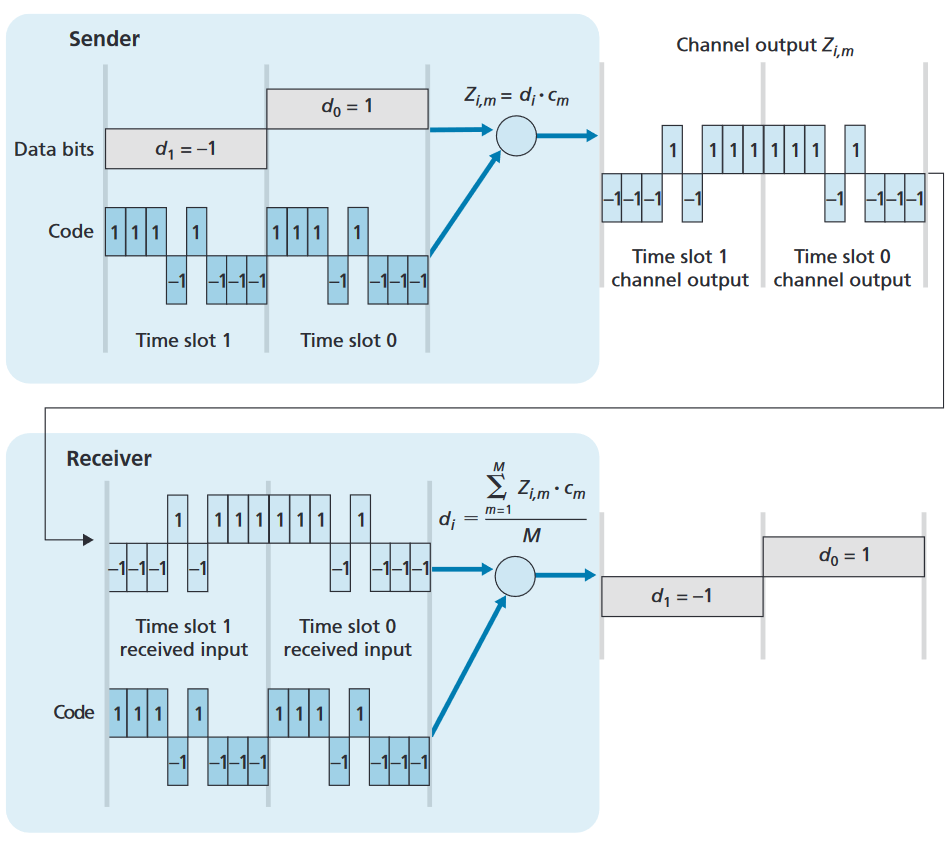
\includegraphics[width=300px]{assets/CDMA.png}\\
				To get the value again it is done by $d_i=\frac{1}{M}\sum\limits_{m=1}^MZ_{i,m}\cdot c_m$\\
				By this the average can be taking and therefore the longer code decrease the chance of a bit error.\\
				Therefore even in case of two signal and the signal is additive, then each receiver will still get the correct value by using the correct code.\\
				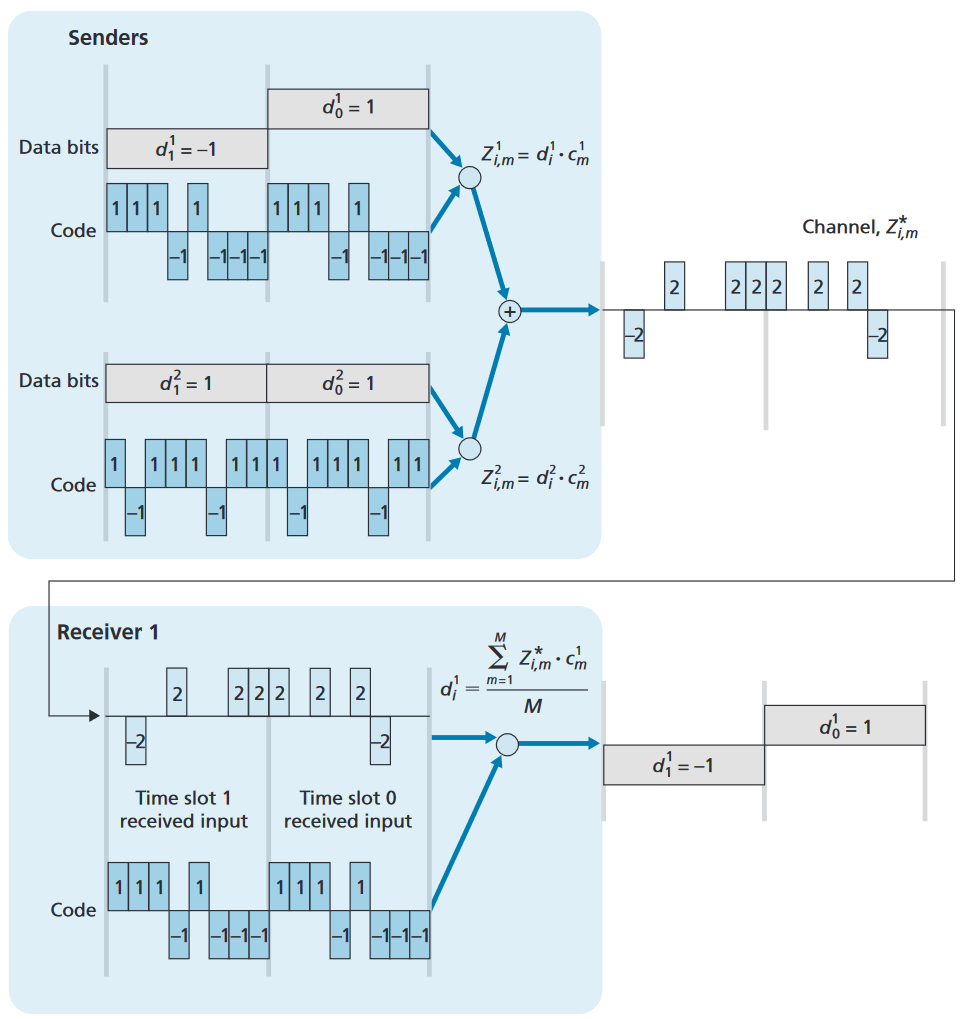
\includegraphics[width=300px]{assets/CDMAInter.png}\\
		\subsection{WiFi: 802.11 Wireless LANs}
			Comes in different standard which changes the frame but is backwards compatible.\\
			WiFi comes in two frequency ranges 2.4-2.485 GHz and 5.1-5.8 GHz, where 2.4 is unlincensed and therefore used more, and 5 GHz does not reach as far on the same power level and suffer more from multipath propagation.\\
			Uses CSMA/CA protocol
			\subsubsection{CSMA/CA protocol}
				Carriere Sense multiple Access is a method for making hosts not transmit in the way of eachother.\\
				Works by the rules: Listen before speaking and if someone else begins talking at the same time stop talking.\\
				CSMA with collision detection (CSMA/CD) is an extenstion to the CSMA.\\
				CSMA works by in case of a collision and a transmitter does not get its acknowledgment it will wait a random interval and then try to retransmit.\\
				CSMA/CD expands upon this such if it reads a signal while transmitting it will stop the transmission and go to waiting, instead of still sending the whole package.\\
				The time interval is choosen in a binary exponential backoff such it starts low and get exponentially larger for every collision.\\
				The efficiency will then be equal $\frac{1}{1+5d_{prop}/d_{trans}}$
		\subsubsection{WiFi wireless LAN Architecture}
			Is a basic serve set (BSS) and contains a one or more wireless stations and central base station known as the access point (AP).\\
			The typical network therefore have a router and AP most often integrated into one unit.\\
			The wireless station has a 6 byte MAC address for connecting, likewise the AP.\\
			Wireless statiosn needs to associate with an AP before it can send or receive network layer data.\\
			An AP has an associated service set identifier (SSID) which identified the AP.\\
			The frequency is the nsplit into smaller ranges for 2.4 GHz there is 11 partially overlapping channels, where channels seperated by four or more channels is non overlapping.\\
			The find an AP a beacon frame is sent periodically, with the APs SSID and MAC address, and devices scans the 11 channels for beacon messages known as passive scanning.\\
			For the device to choose the connected APs the host themselve implements an algorithm not specified.\\
			Active scanning the device sends a broadcasting probe frame which is responded to by the AP.\\
			When connected a DHCP discovery message is send into the subnet through the AP.\\
			The AP can authenticate with different methods.\\
			\begin{itemize}
				\item Devices MAC address
				\item Username and passwords
			\end{itemize}
			This can be handled by an authentication server 
	\subsection{802.11 MAC Protocol}
		There are three different classes of multiple access protocols
		\begin{itemize}
			\item Channel partioning including CDMA
			\item Taking turns
			\item Random access
		\end{itemize}
		\subsubsection{Taking turns}
			Taking turns work by a polling master is choosen, the master make sure that in turn every node is in turn given access to the medium.\\
			This has drawbacks in case of the master occour some error it will stop the whole protocol until a recover is done.\\
			A decentratilized alternative is the token passing protocol, where a fixed order is choosen and once a token is given the host can use the medium and pass on the token after use.\\
			The problem is in case of a host occour an error and does not forward the token it stops the protocol
		\subsubsection{Random access}
			Tries to transmit frames in case of collision wait a random amount of time.\\
			Example is Slotted ALOHA wich retransmit using a probability\\
			The most optimal probabillity is 37\% making 26\% chance of collision\\
			The MAC uses this form of protocol known as CSMA without collision avoidance.\\
			This is due to to host may not detect other networks transmission because they are opposite of the router and therefore the router receive the transmission before the other host known as hidden terminals.\\
			Therefore the WiFI uses a link-layer acknowledgment/retranmisssion (ARQ) scheme.\\
			When the destionation receive a frame that passes the CRC waits a short inter-frame spacing (SIFS) and sends an acknowledment frame.\\
			In case of no ack the host will retransmit.\\
		\subsubsection{Hidden terminals}
			To counteract the problem a reservation of the medium is given by the AP.\\
			A host sends a short request to send (RTS) control frame, and if responded by the AP with a Clear to Send (CTS) frame allows the host to send data.\\
			Collision will be a little problem due to the frames being short.\\
		\subsubsection{Frame}
			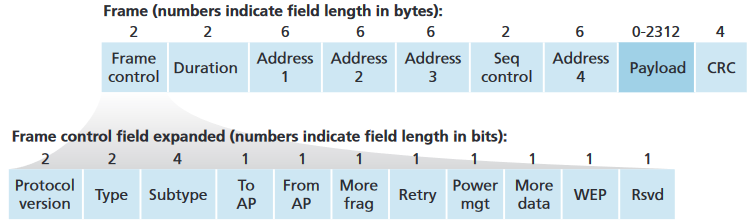
\includegraphics[width=300px]{assets/wifiFrame.png}\\
			Payload up to 2312 bytes, but mostly fewer than 1500 bytes.\\
			The frame has four address field
			\begin{itemize}
				\item Mac address of the wireless station that is to receive the frame
				\item Mac address of the station that transmits the frame
				\item Mac address of the router which connects the subnet to the router
				\item Used for forward frames to each other in ad hoc mode
			\end{itemize}
			Duration used for reservation of the medium.\\
			The type and subtype fields are used to distingiush the association RTS, CTS, ACK and data frames.\\
			To and From field are used to defined meanings of the different address fields.\\
			WEP indicated if encryptions is being used.
		\subsubsection{Mobility in the same IP subnet}
			Mobility between BSSs is straightforward if the BSSs is part of the subnet.
			This can allow the host to keep the IP and all ongoing TCP connections.\\
			Otherwise a new IP is needed through DHCP and will disrupt all TCP connections.\\
		\subsubsection{Advanced features}
			Rate adaption selects the modulation technique.\\
			If an ode sends two frames in a row without receiving an acknowlegment the transmission rate falls back to the next lower rate.\\
			If 10 frames succeedes the increases to a new higher rate.\\
			Power management can be done by managing sleep and wake states.\\
			A node will tell the AP when it goes to sleep by setting a power management bit in the header.\\
			A time in the node is set to wakeup just before the AP beacon time.\\
			The AP then buffers frames for the node, and in the beacon tells if nodes have any buffered frames.\\
			If any then fulkly wakes up otherwise goes back to sleep.\\
		\subsubsection{Personal Area networks: Bluetooth}
			Uses time division multiplexing (TDM) which divides time into time frames and further divides each time frame into N time slots.\\
			Each time slot is then assigned to a node. Time slots size is choosen based on transmission time of a single packet.\\
			TDM eliminates collision and is fair but waste a lot of time in case of nodes not always having to transmit.\\
			It also uses FDM which divides the medium range into channels which a node is assigned to but suffers the same problem as TDM.\\
			Randomized backoff and polling, error detection and corecction and reliable data transfer via ACKS and NAKS.\\
			Uses 2.4 GHz.\\
			During a timeslot of the TDM one of 79 channels is used which is changed in a psudo random way known as frequency hopping spread spectrum (FHSS)\\
	\section{Securing wireless Lans and 4g/5g}
		The wireless nature makes it possible to sniff all packages.\\
		802.11 shoudl handle
		\begin{itemize}
			\item Mutual authentication - verify the identity and access privileges, likewise the device authenticate the nework
			\item Encryption - Using the symmetric key encryption is used in practive since encryption and decryotion must be performed at high speed.
		\end{itemize}
		To process the mutual authentication and encryption-key deriviation
		\begin{enumerate}
			\item Discovery - AP advertise its presence and the forms of authentication and encryotion, the deivce then request specific forms of quth and encryption
			\item Mutual authentication and shared symmetric key derrication - Devices and AP share a common secret (eg password), using this an nonces and cryptographcis hashing
			\item Shared symmetric session key distribution - A protocol will be needed for the authentication server to inform the PA of the shared symmetric symmetric session key
			\item Enrypted communication between mobile device and a remote host via the AP - AES used
		\end{enumerate}
		\subsection{Mutual authentication and shared symmetric session key deriviation}
			The first standard Wired equivalent privacy (WEP) contained security flwas.\\
			WiFi procected access (WPA1) came with message integrit check, and avoided attacks which could infer encryption key after some observation\\
			WPA2 mandated the use of AES symmetric key encryption.\\
			WPA is a four-way handshake protocol that performs both mutual authentication and shared symmetric session-key deriviation.\\
			The handshake goes as
			\begin{enumerate}
				\item Authentication server (AS) generate a nonce and sensd it to the mobile device
				\item Mobile device M receive the nonce generated the symmetric shared session key using the AS nonce and its own nonce and the known secret and MAC address of M and AS, ands ends its own nonce and the AS nonce and secret key in HMAC signed package
			\end{enumerate}
			WPA3 updates attack on the four way handshae by using reused nonce and longer key length among other changes.\\
		\subsection{Authentication and key agreement in 4g/5g}
			The 4g authentication protocol AKA consis of 
			\begin{enumerate}
				\item Authentication request to HSS - device sends its internation mobile subscriber identity (IMSI) which is related to the Mobility Managemenet Entity (MME), MME then sends it to the Hoem subscriver service (HSS)
				\item Authentication resposne from HSS - HSS uses shared secret key to create an authentication token
				\item Authentication response from mobile device - uses the shared secret key to decode the authentication token and sends the answer to the HSS
				\item Mobile device authentication - If a match is done HSS inform the base station and mobile device that it is authorized and sends the base station keys used in the authenticatio ntoken
				\item Data plane and control plane key derrivation - Base and mobile device agree on encryption protocol using the auth key
			\end{enumerate}
			For 5g there were changes to
			\begin{itemize}
				\item Two new protocols for authentication and key agreement, menat for IoT environment and does not need shared secret key
				\item Uses public key cryptography techniques to encrypt a devices permanent identity
			\end{itemize}
	\section{Anonymity and Privacy}
		Anonymity can only somewhat be reached using the protocol looked at so far.\\
		Using IPsec it is possible to anonymice the sender but not the receiver.\\
		It is possible to reach confidentiality with TLS and IPSec (confidentiality has some identificer to pin point the connection unlike anonymous which is simply a connection)\\
		\subsection{Internet}
			Unlike the open internet known as the NFS net, there exist different networks which is also connectable.\\
			The deep web consist of non indexed sites, and therefore will not appear in search engines and the direct url have to be known to access.\\
			The dark web uses different protocol with more encryption and uses multiple hops to get access to sites  not visible on the normal net anonymously.\\
			TOR is a browser used for setting up an onion connection.\\
			It is done by selecting 3 onion nodes, and generating shared key with each.\\
			Then the message is encoded for each three nodes such the first node decodes the first layer and sends it further, until the last node decodes the actual message and sends it to the wanted web server.\\
			The TOR browser defines
			\begin{itemize}
				\item Message length - to ensure that length could not be used to determine where in the chain the message is
				\item Message structure
				\item How to establish keys
				\item How messages is sent
				\item How nodes should decrypt adn forward messages
			\end{itemize}
			Due to the encreased hops and encryption the browser is substantiol slower.\\
			The nodes use trusted guard/entry nodes such an entity can not get enough nodes to determine traffic
		\subsection{Hidden services - Onion websites}
			Onion websites exists on in the nodes, such it never leaves the TOR network.\\
			This achives that either the client or server know eachother if no authentication.\\
			The will ensure privacy in case of a sniffer at the input and output and a client can be correlated to ouput, therefore defeating anonymously.\\
			A hidden service is setup by selecting three random nodes as entry nodes ie nodes which knows the address of the server.\\
			The service is then added to the global hash table (known as DHT distributed on all nodes) as a descriptor with its onion address as key, and the value pair of ip for entry nodes and its public key for authentication.\\
			When a connection is made after the wanted hops it connects to an entry point which essentially forwards, the service then goes to the last node known as the redezvous point (RP) of the chain before the entry point and sends the response through its own number of hops.\\
			The onion address comes in different versions
			\begin{itemize}
				\item Version 1 - Generated from public key
				\item Version 2 - First half of base32 encoded SHA-1 hash of public key from 1024 RSA 
				\item Version 3 (standard) - Is now 56 characters long, uses SHA-3 instead and curve25519 instead of RSA, making it more private and robust
			\end{itemize}
			
			
			
			
\end{document}
